% questions.tex —— 1986 年·广东卷·文史类 · 题目内容片段（无答案）
% 由 tools/generate_projects.py 依来源总账自 1986/1986_数学真题_广东文_试题.md 生成，勿手改（改源 MD 后重跑）


\begin{gktip}
\textbf{来源说明}：本题面依据固定源 PDF《一九八六年广东省高考数学（文史类）试题与解答》PDF 第 1—9 页逐题转录，书中页码为 260—268；PDF 第 10—17 页为解答和答案。固定源为扫描 PDF，无可用文本层。下列题面以试题页为准，答案和解析由本库独立复算，不声称代表官方发布版本。

\textbf{版式与异文说明}：第 14 题的 $\sin1,\cos1,\operatorname{tg}1$ 无度数符号，按弧度解释；第 7 题定义域右端为闭区间 $8]$。第 2 题第（2）小题的乘号在固定源中呈方框缺字形，照录为 $\square$。

\textbf{图形说明}：第二卷第二题的题面图按固定源重绘为 TikZ 矢量图，仅标出原图中的 $S,A,B,C$；隐藏棱 $AC$ 用虚线表示。解析所用辅助点另见解析版图稿。
\end{gktip}

\begin{question}
\gkti{1}（本题满分 50 分）本题共有 25 个小题。每一个小题都给出代号为 $A\text{、}B\text{、}C\text{、}D\text{、}E$ 的五个结论，其中只有一个结论是正确的。请把正确结论的代号选出，并在答题卷中的相应位置上涂黑（每个小题选对得 2 分，不选、选错或者选出的代号超过一个，一律得 0 分）。

\Needspace{5\baselineskip}
（1） 方程

\nopagebreak[4]
\[
2^{2x+1}-9\cdot2^x+4=0
\]

的解集是\mbox{（　　）}

（A）$\{2\}$　　（B）$\{-1\}$　　（C）$\{\frac12\}$

（D）$\{-1,2\}$　　（E）$\{\frac12,2\}$

（2） 若直线过点 $(\sqrt3,-3)$ 且倾斜角为 $30^\circ$，则该直线的方程为\mbox{（　　）}

（A）$y=\sqrt3x-6$　　（B）$y=\dfrac{\sqrt3}{3}x+4$

（C）$y=\dfrac{\sqrt3}{3}x-4$　　（D）$y=\dfrac{\sqrt3}{3}x+2$

（E）$y=\sqrt3x+4\sqrt3$

\Needspace{5\baselineskip}
（3） 两平行线

\nopagebreak[4]
\[
3x+4y-12=0,\qquad 6x+8y+6=0
\]

间的距离是\mbox{（　　）}

（A）$\dfrac95$　　（B）$-3$　　（C）$6$　　（D）$18$　　（E）$3$

\Needspace{5\baselineskip}
（4） 直角坐标方程

\nopagebreak[4]
\[
x^2+2x-y^2+2y=0
\]

所表示的曲线是\mbox{（　　）}

（A）椭圆　　（B）双曲线　　（C）互相平行的两直线

（D）互相垂直的两直线　　（E）一个点

\Needspace{5\baselineskip}
（5） 若

\nopagebreak[4]
\[
\cos2\alpha=-\frac35,\qquad \alpha\in\left[0,\frac\pi2\right],
\]

则 $\sin\alpha$ 等于\mbox{（　　）}

（A）$\dfrac{2\sqrt5}{5}$　　（B）$\dfrac{\sqrt5}{5}$　　（C）$\dfrac{\sqrt5}{10}$

（D）$\dfrac15$　　（E）$\dfrac25$

\Needspace{5\baselineskip}
（6） 若

\nopagebreak[4]
\[
P_m^3=6C_m^4,
\]

则 $m=$\mbox{（　　）}

（A）6　　（B）7　　（C）8　　（D）9　　（E）10

\Needspace{5\baselineskip}
（7） 函数

\nopagebreak[4]
\[
y=\log_{\frac12}x,\qquad x\in(0,8]
\]

的值域是\mbox{（　　）}

（A）$[-3,+\infty)$　　（B）$[3,+\infty)$　　（C）$(-\infty,-3]$

（D）$(-\infty,3]$　　（E）$(0,+\infty)$

\Needspace{5\baselineskip}
（8） 若

\nopagebreak[4]
\[
A=\{x\mid |x-1|<2\},
\]

\nopagebreak[4]
\[
B=\left\{x\middle|\frac{x-2}{x}>0\right\},
\]

则 $A\cap B=$\mbox{（　　）}

（A）$\{x\mid -1<x<3\}$　　（B）$\{x\mid x<0\text{ \text{或} }x>2\}$

（C）$\{x\mid -1<x<0\}$　　（D）$\{x\mid -1<x<0\text{ \text{或} }2<x<3\}$

（E）$\{x\mid 0<x<2\}$

（9） 从 8 名男医生和 7 名女医生中选 5 人组成一个医疗小组。如果这个小组中至少有 2 名男医生和至少有 2 名女医生，则不同选法的种数是\mbox{（　　）}

（A）$(C_8^3+C_7^2)(C_8^2+C_7^3)$

（B）$(C_8^3+C_7^2)+(C_8^2+C_7^3)$

（C）$C_8^2C_7^3$　　（D）$C_8^2C_7^2C_{11}^1$

（E）$C_8^2C_7^3+C_8^3C_7^2$

\Needspace{5\baselineskip}
（10） 不等式

\nopagebreak[4]
\[
\frac{x^2-x-6}{-x^2-1}>0
\]

的解集是\mbox{（　　）}

（A）$\{x\mid -2<x<3\}$　　（B）$\{x\mid x<-2\text{ \text{或} }x>3\}$

（C）$\{x\mid -2<x<+\infty\}$　　（D）$\{x\mid 3<x<+\infty\}$

（E）$\{x\mid -3<x<2\}$

（11） 复数 $\sin95^\circ+i\cos95^\circ$ 的一个辐角是\mbox{（　　）}

（A）$95^\circ$　　（B）$-85^\circ$　　（C）$5^\circ$　　（D）$85^\circ$　　（E）$-5^\circ$

（12） 侧面为等边三角形的正三棱锥，其侧面与底面所成二面角的余弦值是\mbox{（　　）}

（A）$\dfrac12$　　（B）$\dfrac{\sqrt2}{3}$　　（C）$\dfrac13$

（D）$\dfrac{\sqrt2}{2}$　　（E）$\dfrac{\sqrt3}{2}$

（13） 若圆台下底面半径为 4，上底面半径为 1，母线长为 $3\sqrt2$，则其体积为\mbox{（　　）}

（A）$15\pi$　　（B）$21\pi$　　（C）$25\pi$　　（D）$63\pi$　　（E）$21\sqrt2\pi$

（14） $\sin1,\cos1,\operatorname{tg}1$ 的大小关系是\mbox{（　　）}

（A）$\sin1<\cos1<\operatorname{tg}1$　　（B）$\operatorname{tg}1<\sin1<\cos1$

（C）$\cos1<\operatorname{tg}1<\sin1$　　（D）$\sin1<\operatorname{tg}1<\cos1$

（E）$\cos1<\sin1<\operatorname{tg}1$

\Needspace{12\baselineskip}

\Needspace{5\baselineskip}
（15） 若

\nopagebreak[4]
\[
0<\alpha<\frac\pi2,\qquad 0<\beta<\frac\pi2,
\]

\nopagebreak[4]
\[
\text{且}\quad \operatorname{tg}\alpha=\frac17,\qquad \operatorname{tg}\beta=\frac34,
\]

则 $\alpha+\beta=$\mbox{（　　）}

（A）$\dfrac\pi6$　　（B）$\dfrac\pi4$　　（C）$\dfrac\pi3$

（D）$\dfrac\pi2$　　（E）$\dfrac34\pi$

\Needspace{5\baselineskip}
（16） 计算下式：

\nopagebreak[4]
\[
\frac{1+\sin2\theta-\cos2\theta}
{1+\sin2\theta+\cos2\theta}
\]

等于\mbox{（　　）}

（A）$\operatorname{tg}\theta$　　（B）$\operatorname{ctg}\theta$　　（C）$\sin\theta$

（D）$2\sin\theta$　　（E）$\sin2\theta$

\Needspace{5\baselineskip}
（17） 若 $\beta\in[0,2\pi)$，且

\nopagebreak[4]
\[
\sqrt{1-\cos^2\beta}+\sqrt{1-\sin^2\beta}
=\sin\beta-\cos\beta,
\]

则 $\beta$ 的取值范围是\mbox{（　　）}

（A）$\left[0,\dfrac\pi2\right]$　　（B）$\left[\dfrac\pi2,\pi\right]$

（C）$\left[\pi,\dfrac{3\pi}2\right]$　　（D）$\left[\dfrac{3\pi}2,2\pi\right)$

（E）$\left[\dfrac\pi4,\dfrac{5\pi}4\right]$

\Needspace{5\baselineskip}
（18） 求值：

\nopagebreak[4]
\[
\operatorname{ctg}\frac98\pi
\]

的值是\mbox{（　　）}

（A）$\sqrt2-1$　　（B）$\sqrt3-2$　　（C）$-1-\sqrt2$

（D）$\sqrt2+1$　　（E）$3-\sqrt2$

\Needspace{5\baselineskip}
（19） 函数

\nopagebreak[4]
\[
y=-2\cos^2x-2\sin x+\frac92
\]

的最小值是\mbox{（　　）}

（A）$\dfrac52$　　（B）$2$　　（C）$\dfrac92$　　（D）$3$　　（E）$\dfrac12$

\Needspace{5\baselineskip}
（20） 椭圆

\nopagebreak[4]
\[
\frac{(x+1)^2}{4}+y^2=1
\]

\Needspace{5\baselineskip}
与抛物线

\nopagebreak[4]
\[
y=1-(x+1)^2
\]

的交点个数是\mbox{（　　）}

（A）0　　（B）1　　（C）2　　（D）3　　（E）4

\Needspace{5\baselineskip}
（21） 若动圆与圆

\nopagebreak[4]
\[
(x+2)^2+y^2=4
\]

相外切且与直线 $x=2$ 相切，则动圆圆心的轨迹方程是\mbox{（　　）}

（A）$y^2+8x=0$　　（B）$y^2-8x=0$　　（C）$y^2-12x+12=0$

（D）$y^2+12x-12=0$　　（E）$y^2-6x+6=0$

\Needspace{5\baselineskip}
（22） 过点 $A(1,-2)$ 及椭圆

\nopagebreak[4]
\[
\frac{x^2}{6}+\frac{y^2}{5}=1
\]

的两个焦点的圆的方程是\mbox{（　　）}

（A）$x^2+2x+y^2=4$　　（B）$x^2-2x+y^2=3$

（C）$x^2+y^2+2y=1$　　（D）$x^2+y^2-2y=1$

（E）$x^2+y^2+2y=0$

\Needspace{5\baselineskip}
（23） 函数

\nopagebreak[4]
\[
y=\cos x+\sin x,\qquad x\in[0,2\pi)
\]

的单调下降区间是\mbox{（　　）}

（A）$\left[\dfrac\pi2,\dfrac{3\pi}2\right]$

（B）$\left[\dfrac{3\pi}4,\dfrac{7\pi}4\right]$

（C）$[\pi,2\pi)$　　（D）$\left[\dfrac\pi4,\dfrac{3\pi}4\right]$

（E）$\left[\dfrac\pi4,\dfrac{5\pi}4\right]$

（24） 若点 $A$ 的坐标为 $(3,2)$，$F$ 为抛物线 $y^2=2x$ 的焦点，点 $P$ 在该抛物线上移动，为使 $|PA|+|PF|$ 取最小值，点 $P$ 的坐标应为\mbox{（　　）}

（A）$(0,0)$　　（B）$(1,1)$　　（C）$(2,2)$　　（D）$(\frac12,1)$　　（E）$(1,\sqrt2)$

\Needspace{5\baselineskip}
（25） 若函数

\nopagebreak[4]
\[
y=f(x)
\]

\Needspace{5\baselineskip}
是函数

\nopagebreak[4]
\[
y=1-\sqrt{1-x^2},\qquad -1\le x\le0
\]

的反函数，则 $y=f(x)$ 的图象大致形状是\mbox{（　　）}

\begin{gktip}
固定源第 4 页在题干之后的 A—E 图形选项区域完全空白；本题保留题干和答案表信息，不凭空补画选项图。
\end{gktip}

\end{question}
\begin{question}
\gkti{2}（本题满分 30 分）本题共有 10 个小题，每一个小题满分 3 分，只要求直接写出结果。

\Needspace{5\baselineskip}
（1） 函数

\nopagebreak[4]
\[
y=2\log_3x\qquad(x>0)
\]

的反函数是 $\underline{\hspace{2em}}$。

\Needspace{5\baselineskip}
（2） 将极坐标方程

\nopagebreak[4]
\[
\rho=\operatorname{tg}\theta\ \square\ \sec\theta
\]

化为直角坐标方程，得 $\underline{\hspace{2em}}$。

\begin{gktip}
固定源中的乘法位置显示为方框缺字形 $\square$，按题意和解答页解释为乘法，但题面记录不替换该字形。
\end{gktip}

\Needspace{5\baselineskip}
（3） 若球内切于圆柱，则它们的表面积之比

\nopagebreak[4]
\[
S_{\text{\text{圆柱全}}}:S_{\text{\text{球}}}
\]

的值是 $\underline{\hspace{2em}}$。

\Needspace{5\baselineskip}
（4） 中心在原点的双曲线，若其实半轴长为 2，一条准线的方程为

\nopagebreak[4]
\[
x=-\frac12,
\]

则该双曲线的离心率的值是 $\underline{\hspace{2em}}$。

\Needspace{5\baselineskip}
（5） 设函数 $y=\lg(x^2-x-2)$ 的定义域为 $A$，函数

\nopagebreak[4]
\[
y=\sqrt{\frac{x+2}{1-x}}
\]

的定义域为 $B$，则 $A\cap B=$ $\underline{\hspace{2em}}$。

（6） 若 $f\left(1+\frac{1}{x}\right)=\frac{1}{x^2}-1$，则 $f(x)=$ $\underline{\hspace{2em}}$。

\Needspace{5\baselineskip}
（7） 计算下式：

\nopagebreak[4]
\[
(2x-1)^5
\]

的展开式中各项系数的绝对值的和为 $\underline{\hspace{2em}}$。

\Needspace{5\baselineskip}
（8） 求极限：

\nopagebreak[4]
\[
\lim_{n\to\infty}\sqrt n\left(\sqrt{n+1}-\sqrt n\right)
=\underline{\hspace{2em}}\text{。}
\]

\Needspace{5\baselineskip}
（9） 若等差数列 $\{a_n\}$ 的公差为正数，且

\nopagebreak[4]
\[
a_3a_7=-12,\qquad a_4+a_6=-4,
\]

则前 20 项之和 $S_{20}=$ $\underline{\hspace{2em}}$。

\Needspace{5\baselineskip}
（10） 当 $a$ 在 $(-\infty,0)$ 内变化时，要使过三点

\nopagebreak[4]
\[
O(0,0),\qquad A(-4,0),\qquad B(-2,a)
\]

的圆的圆心在 $\triangle AOB$ 内（包括边界），则 $a$ 允许取的最大值是 $\underline{\hspace{2em}}$。

\end{question}
\begin{question}
\gkti{3}（本题满分 8 分）设有对数方程

\nopagebreak[4]
\[
\lg(ax)=2\lg(x-1).
\]

（1） 当 $a=2$ 时，解该对数方程；

（2） 讨论当 $a$ 在什么范围内取值时，该对数方程有解，并求出它的解。

\end{question}
\begin{question}
\gkti{4}（本题满分 6 分）设

\nopagebreak[4]
\[
y=\frac{1-\sin\theta\cos\theta}
{1+\sin\theta\cos\theta},
\]

当 $\theta$ 在 $[0,\pi]$ 上分别取何值时，$y$ 取得最大值和最小值。

\end{question}
\begin{question}
\gkti{5}（本题满分 12 分）写出棣莫弗定理并用数学归纳法加以证明。

\Needspace{0.4\textheight}
\end{question}
\begin{question}
\gkti{6}（本题满分 12 分）在三棱锥 $S-ABC$ 中，平面 $SAC\perp ABC$，$AB=AC=a$，$\angle BAC=90^\circ$，$SA=SC=b$。求：

（1） 棱 $SB$ 与平面 $ABC$ 所成角的正切；

（2） 三棱锥被过 $S$ 且与 $BC$ 垂直的平面所截得的截面面积。
\nopagebreak[4]
\begin{center}% 1986 年广东卷文史类第 6 题：固定源题面三棱锥图（仅 S/A/B/C）
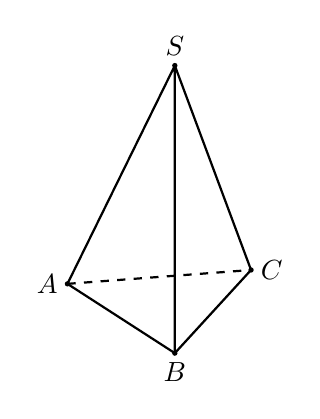
\begin{tikzpicture}[scale=0.88,>=stealth]
  \coordinate (A) at (0,0);
  \coordinate (B) at (1.55,-1.0);
  \coordinate (C) at (2.65,0.2);
  \coordinate (S) at (1.55,3.15);

  \draw[thick] (A)--(B)--(C);
  \draw[dashed,thick] (A)--(C);
  \draw[thick] (S)--(A) (S)--(B) (S)--(C);
  \fill (A) circle (1.1pt) node[left] {$A$};
  \fill (B) circle (1.1pt) node[below] {$B$};
  \fill (C) circle (1.1pt) node[right] {$C$};
  \fill (S) circle (1.1pt) node[above] {$S$};
\end{tikzpicture}
\end{center}
\nopagebreak[4]
\end{question}
\begin{question}
\gkti{7}（本题满分 12 分）已知椭圆 $C$ 的直角坐标方程为

\nopagebreak[4]
\[
\frac{x^2}{4}+\frac{y^2}{3}=1,
\]

\Needspace{5\baselineskip}
试确定 $m$ 的取值范围，使得对于直线

\nopagebreak[4]
\[
y=4x+m,
\]

椭圆 $C$ 上有不同的两点关于该直线对称。

\end{question}